\begin{exercice}
   \phantom{rrr}

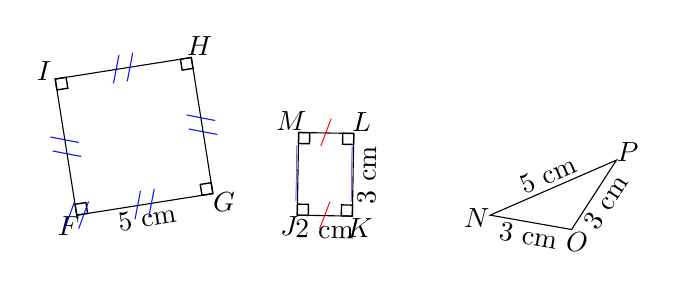
\begin{tikzpicture}[baseline,scale = 0.35]

    \tikzset{
      point/.style={
        thick,
        draw,
        cross out,
        inner sep=0pt,
        minimum width=5pt,
        minimum height=5pt,
      },
    }
    %\clip (-2,-3) rectangle (22,7);


   \draw[color={black}] (0,0)--(4.938441702975689,0.7821723252011543)--(4.156269377774535,5.720614028176843)--(-0.782172325201154,4.938441702975689)--cycle;
	
	\draw [color={black}] (-0.2938926261462367,-0.4045084971874737) node[anchor = center,scale=1] {$F$};
	\draw [color={black}] (5.342950200163163,0.4882796990549174) node[anchor = center,scale=1] {$G$};
	\draw [color={black}] (4.450162003920772,6.125122525364317) node[anchor = center,scale=1] {$H$};
	\draw [color={black}] (-1.1866808223886278,5.232334329121926) node[anchor = center,scale=1] {$I$};
	\draw[color={black},line width = 0.5] (4.938441702975689,0.7821723252011543)--(4.543366366737634,0.719598539185062)--(4.480792580721541,1.1146738754231174)--(4.875867916959597,1.1772476614392093)--cycle;
	\draw[color={black},line width = 0.5] (-0.782172325201154,4.938441702975689)--(-0.7195985391850617,4.543366366737634)--(-0.3245232029470062,4.6059401527537265)--(-0.3870969889630989,5.001015488991782)--cycle;
	\draw[color={black},line width = 0.5] (4.156269377774535,5.720614028176843)--(3.76119404153648,5.658040242160751)--(3.823767827552573,5.262964905922695)--(4.218843163790628,5.325538691938788)--cycle;
	\draw[color={black},line width = 0.5] (0,0)--(0.3950753362380551,0.06257378601609234)--(0.3325015502219627,0.45764912225414744)--(-0.06257378601609231,0.3950753362380551)--cycle;
	\draw [color={blue}] (2.4692208514878446,0.39108616260057716) node[anchor = center, rotate = 9] {//};
   \draw [color={blue}] (4.547355540375112,3.2513931766889987) node[anchor = center, rotate = -81] {//};
   \draw [color={blue}] (1.6870485262866906,5.329527865576266) node[anchor = center, rotate = -351] {//};
   \draw [color={blue}] (-0.391086162600577,2.4692208514878446) node[anchor = center, rotate = -81] {//};
   \draw [color={blue}] (0,0) node[anchor = center, rotate = 0] {//};

	\draw [color={black}] (2.5474380840079602,-0.10275800769699167) node[anchor = center, rotate = -351] {5 cm};
	\draw[color={black}] (8,0)--(9.999695390312782,-0.03490481287456702)--(10.052052609624633,2.9646382725946063)--(8.052357219311851,2.999543085469173)--cycle;
	
	\draw [color={black}] (7.715431503694181,-0.4111213578862629) node[anchor = center,scale=1] {$J$};
	\draw [color={black}] (10.269742606705556,-0.45570702403619356) node[anchor = center,scale=1] {$K$};
	\draw [color={black}] (10.336621105930453,3.3757596304808692) node[anchor = center,scale=1] {$L$};
	\draw [color={black}] (7.782310002919077,3.4203452966308) node[anchor = center,scale=1] {$M$};
	\draw[color={black},line width = 0.5] (9.999695390312782,-0.03490481287456702)--(9.599756312250225,-0.027923850299653614)--(9.606737274825138,0.3720152277629035)--(10.006676352887695,0.3650342651879895)--cycle;
	\draw[color={black},line width = 0.5] (10.052052609624633,2.9646382725946063)--(10.04507164704972,2.5646991945320496)--(9.645132568987163,2.5716801571069623)--(9.652113531562076,2.97161923516952)--cycle;
	\draw[color={black},line width = 0.5] (8.052357219311851,2.999543085469173)--(8.452296297374408,2.9925621228942596)--(8.445315334799496,2.5926230448317025)--(8.045376256736938,2.5996040074066165)--cycle;
	\draw[color={black},line width = 0.5] (8,0)--(8.006980962574913,0.3999390780625565)--(8.40692004063747,0.39295811548764387)--(8.399939078062557,-0.006980962574913407)--cycle;
	\draw [color={red}] (8.99984769515639,-0.01745240643728351) node[anchor = center, rotate = -1] {/};
   \draw [color={red}] (9.052204914468241,2.9820906790318897) node[anchor = center, rotate = -1] {/};

	\draw [color={blue}] (10.025873999968708,1.4648667298600198) node[anchor = center, rotate = 89] {||};
   \draw [color={blue}] (8.026178609655926,1.4997715427345866) node[anchor = center, rotate = -271] {||};

	\draw [color={black}] (8.991121491937749,-0.5173762540154792) node[anchor = center, rotate = -1] {2 cm};
	\draw [color={black}] (10.525797847546903,1.4561405266413778) node[anchor = center, rotate = -271] {3 cm};
	\draw[color={black}] (15,0)--(17.954423259036624,-0.520944533000791)--(19.58330384659268,1.9983307658665281)--cycle;
	
	\draw [color={black}] (14.509335758423742,-0.0961696523774262) node[anchor = center,scale=1] {$N$};
	\draw [color={black}] (18.154256335623277,-0.9792749176600588) node[anchor = center,scale=1] {$O$};
	\draw [color={black}] (19.987682609739608,2.2924018727705606) node[anchor = center,scale=1] {$P$};
	\draw [color={black}] (16.390387540684845,-0.7528761430064994) node[anchor = center, rotate = -10] {3 cm};
	\draw [color={black}] (19.18874276929254,0.4672130185068584) node[anchor = center, rotate = -302.89] {3 cm};
	\draw [color={black}] (17.09181884670969,1.4574957675925326) node[anchor = center, rotate = 23.56] {5 cm};

\end{tikzpicture}
\begin{enumerate}
   \begin{spacing}{1.5}
      \item Calculer le périmètre du carré en cm
      \item Calculer le périmètre du rectangle en cm
      \item Calculer le périmètre du triangle rectangle en cm
   \end{spacing}
\end{enumerate}

   \hrefMathalea{https://coopmaths.fr/mathalea.html?ex=6M11-3,i=0&v=l}
 \end{exercice}

 \begin{corrige}
   \begin{enumerate}
      \begin{spacing}{2}
         \item \\
      $\mathcal{P}_{FGHI}=4\times 5~\text{cm}=20~\text{cm}$
         \item \\
      $\mathcal{P}_{JKLM}=2\times 2~\text{cm} + 2\times3~\text{cm}=10~\text{cm}$
         \item \\
      $\mathcal{P}_{NOP}=3~\text{cm} + 5~\text{cm} + 3~\text{cm} =11~\text{cm}$
      \end{spacing}
   \end{enumerate}
 \end{corrige}